\chapter{Evaluierung}



\section{Stormmessung}

Zur Qualitätsbewertung der Stommessung wird das Fahrzeug aufgebockt. 
Das Fahrzeug befand sich während aller Messungen im Akkubetrieb, bei ca. 16,8V Akkuspannung.
Motor wurde, soweit nicht anders beschrieben mit einem PWM-Tastgrad von 30:256 angesteuert.
Zur Beurteilung der Messergebnisse wurden Messungen an diversen Punkten vorgenommen und mit der Ausgabe des Mikrocontrollers verglichen.

Zuerst wurde dazu die Spannung direkt am Shuntwiderstand gemessen.
Dabei kann der periodische Ansteig der Spannung am Shunt beobachtet werden, zu sehen in \cref{fig:filter_eingang}. Die Spannung am Shunt ist Proportional zum Storm durch den Motor.

\begin{figure}[H]
\centering
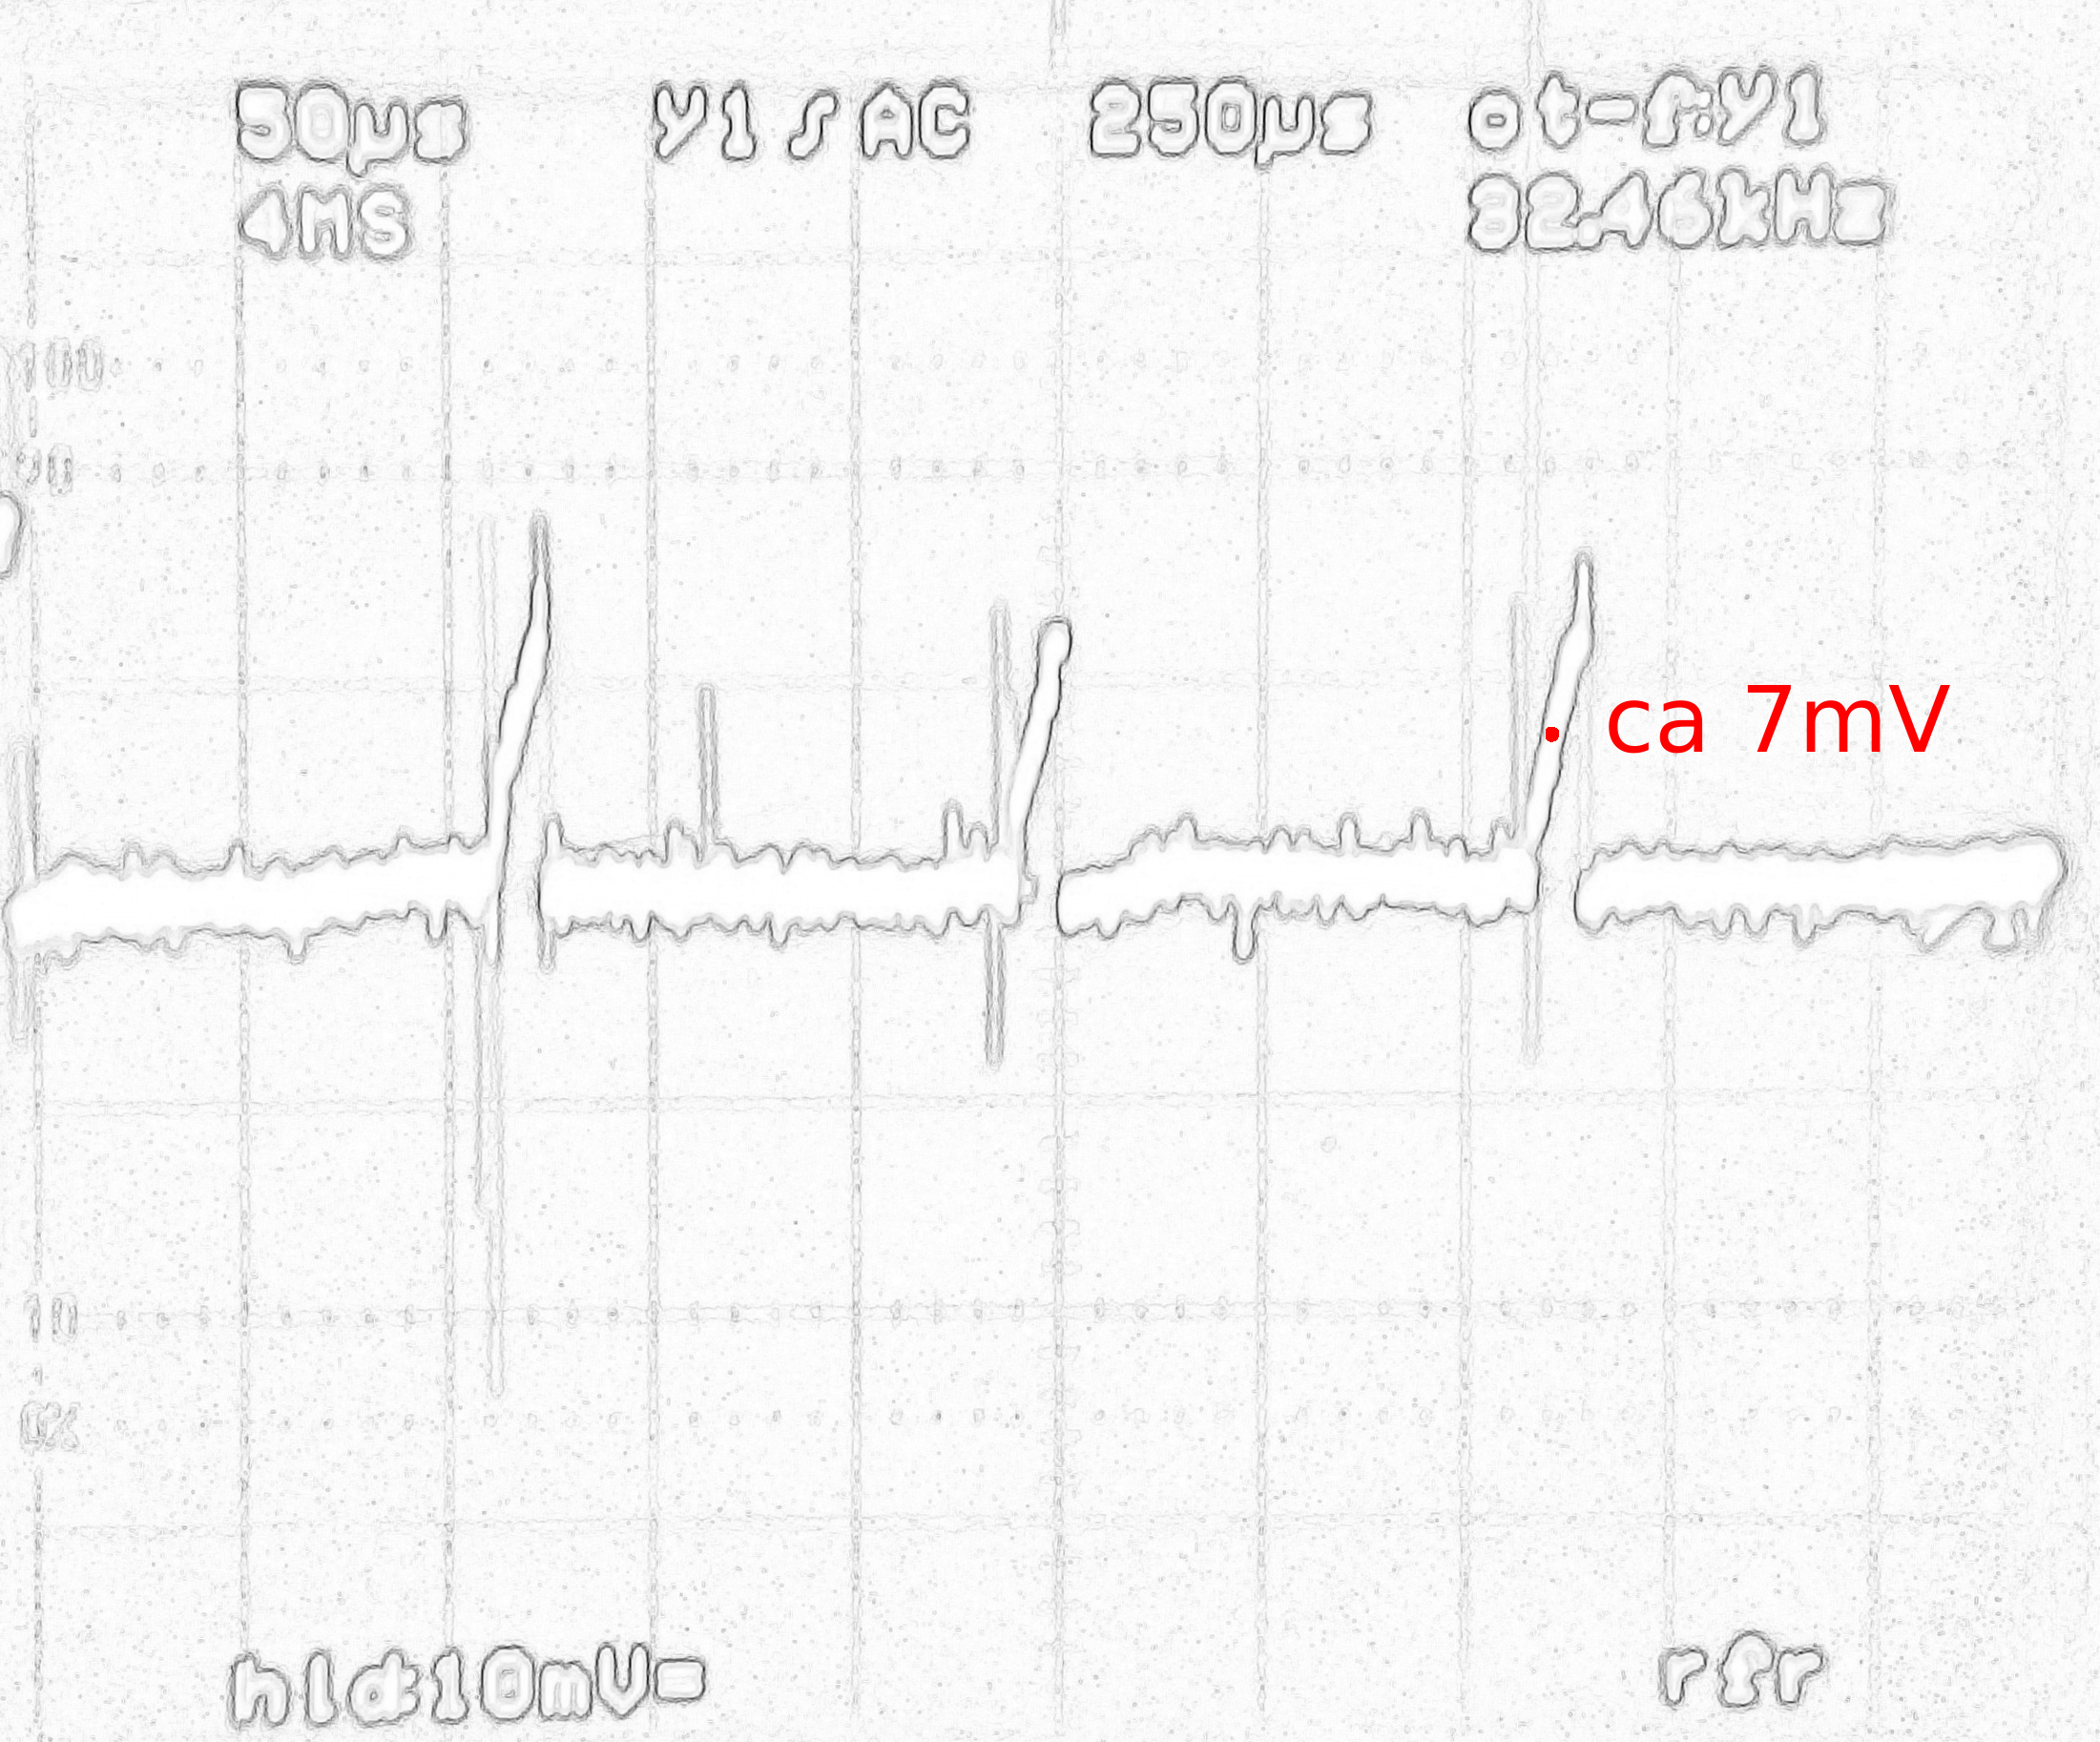
\includegraphics[width=.8\textwidth]{filter_eingang_mak.png}\\
\caption{Spannung am Shunt}%
\label{fig:filter_eingang}
\end{figure}

Die mittlere Spannung aus \cref{fig:filter_eingang} lässt sich abschätzen, in dem die Spannug in der Mitte eines Impulses abliest und sie mit dem Tastverhältnis multipliziert.
$\SI{7}{\mV}\cdot\frac{30}{256}=\SI{0,82}{\mV} $
Mit Hilfe dieses Mittelwertes können wir grob abschätzen ob der nachfolgende Filter seine Funktion erfolgreich erfüllt.


Als nächstes wird die Spannung nach der Filterschaltung direkt am Operationsversärker gemessen. Es fällt auf das das Signal trotz Teifpass noch Störungen in Form des Motorstromes enthält.
Dies ist eine Auswirkung der gestörten Betriebsspannung, welche später untersucht wird.


\begin{figure}[H]
\centering
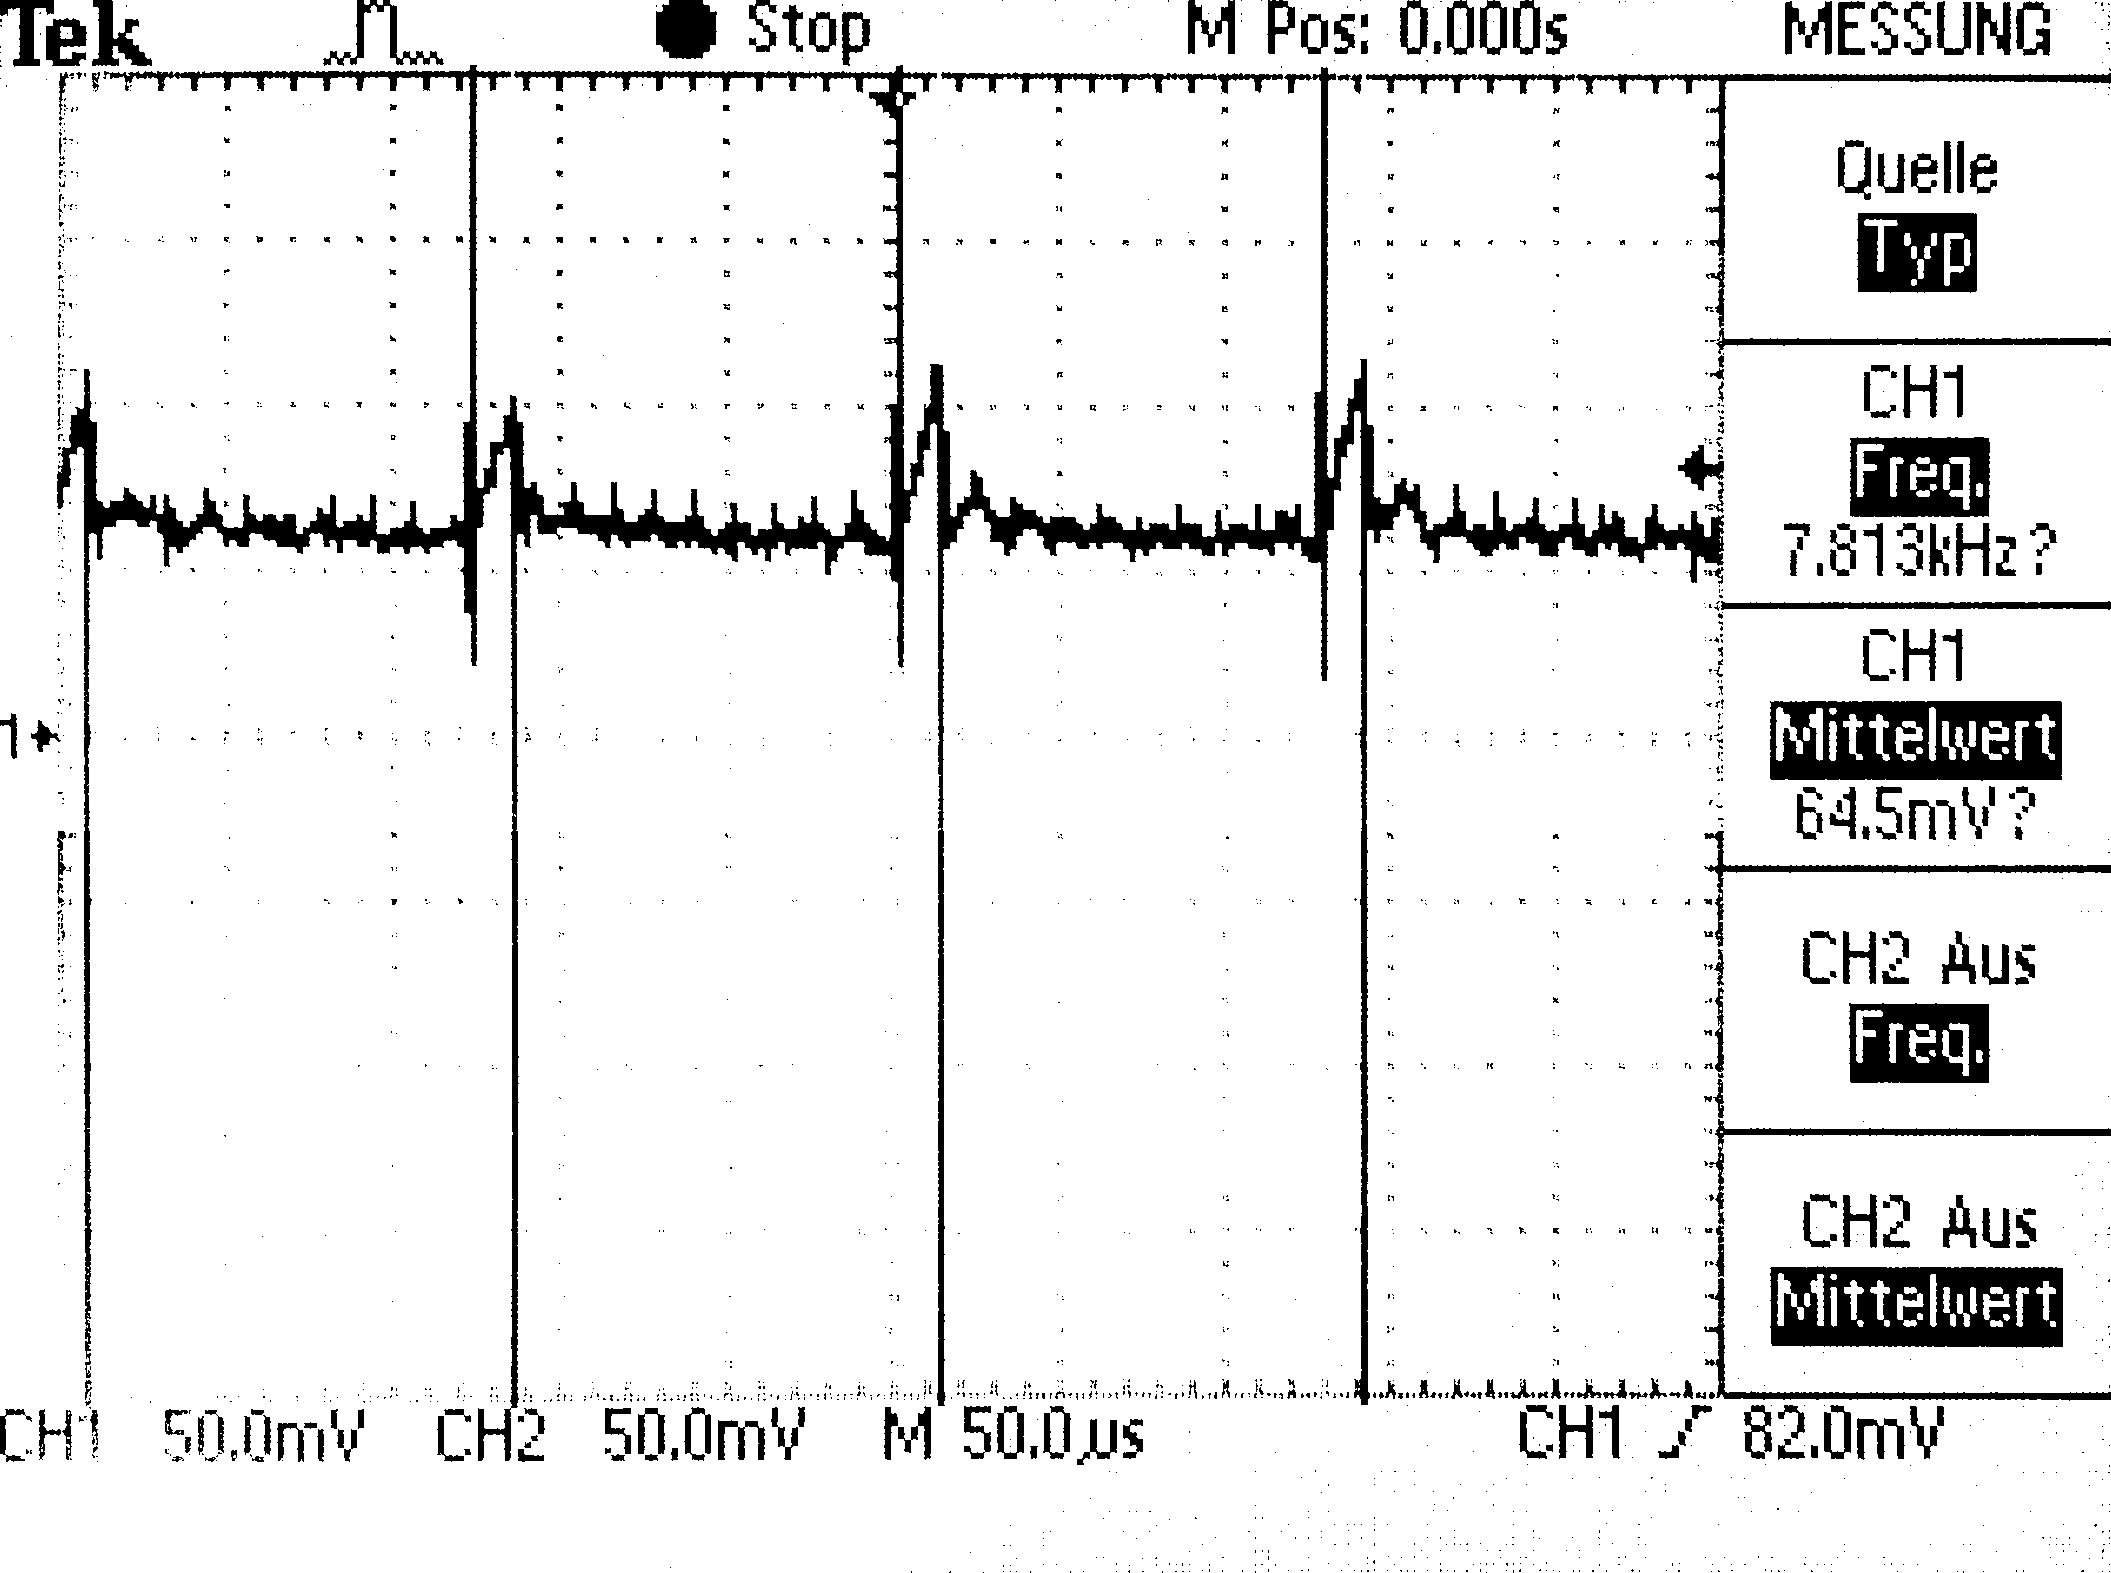
\includegraphics[width=.8\textwidth]{filter_ausgang.png}\\
\caption{Spannung nach dem Filter}%
\label{fig:filter_ausgang}
\end{figure}


Wie in \cref{fig:filter_ausgang} zu sehen wurde die Spannung erfolgreich verstärkt und hat etwa eine Spannung von \SI{40}{\mV}. Dividiert durch den Verstärkungsfaktor 48, ergibt sich eine Spannung von 
\SI{0,83}{\mV}. Welche sehr nahe an dem vorher abgeschätzten Wert von \SI{0,82}{\mV} liegt. Der Strom lässt sich nun mit Hilfe des ohmnschen Gesetzes $U=R\cdot I$ errechnen.
\begin{align*}
I=\frac{\SI{0,83}{\mV}}{\SI{0,005}{\ohm}}=\SI{166,7}{\mA}
\end{align*}

Der vom Microcontroller ausgegebenne Strom beträgt im Mittel \SI{156,1}{\mA}.

Zur weiteren Bewertung der Messung wurden jeweils ca 1000 Samples an Daten zu unterschiedlichen PWM-Tastgraden aufgezeichnet.
Dabei soll untersucht werden, ob die Qualität der Messwerte mir zunehmender Geschwindigkeit stabil bleibt.
Die Ergebnisse der Messungen sind in \cref{tab:current_noload} zu sehen.

\begin{table}[H]
  \centering
  \begin{tabularx}{\textwidth}{|X|r|r|}
    \hline
    Tastgrad & Erwartungswert [A] & Standardabweichung [A]  \\ \hline \hline
    10 & 0.0044 & 0.0212\\ \hline
    20 & 0.0730 & 0.0214\\ \hline
    30 & 0.1600 & 0.0215\\ \hline
    40 & 0.2629 & 0.0214\\ \hline
    50 & 0.3653 & 0.0185\\ \hline
    60 & 0.4720 & 0.0231\\ \hline

  \end{tabularx}
  \caption{Motorstorm im Leerlauf}%
  \label{tab:current_noload}
\end{table}

Die Standardabweichung der Messwerte scheint stabil zu bleiben. Da der Strom sich in diesen Messungen in einem sehr niedrigen Bereich befindet, wurden
die Messungen erneut unter Last durchgeführt, der Motor befand sich währenddessen im Kurzschlussbetrieb.

\begin{table}[H]
  \centering
  \begin{tabularx}{\textwidth}{|X|r|r|}
    \hline
    Tastgrad & Erwartungswert [A] & Standardabweichung [A]  \\ \hline \hline
    10 & 0.0454 & 0.0183\\ \hline
    20 & 0.4635 & 0.0243\\ \hline
    30 & 1.1694 & 0.0338\\ \hline
    40 & 1.9822 & 0.0563\\ \hline
    50 & 3.8737 & 0.0477\\ \hline
    60 & 4.7023 & 0.0706\\ \hline
  \end{tabularx}
  \caption{Motorstrom unter Last}%
  \label{tab:current_load}
\end{table}

Der Tabelle \ref{tab:current_load} kann leicht entnommen werden, das die Ströme unter last stark ansteigen. Die Standardabweichung steigt im Verhältnis zum Strom nur leicht.
So dass die Streuung der Messung mit steigendem Strom zwar zunimmt, die relative Abweichung der Werte jedoch nicht steigt.


\section{Spannungsversorgung}

Während der Untersuchung der Strommessung sind Störungen im Ausgabesignal der Filterschaltung festgestellt wurden. Um die Ursache der Störung zu finden wurde die Spannungsversorgung
des Fahrzeuges untersucht.

\begin{figure}[H]
\centering
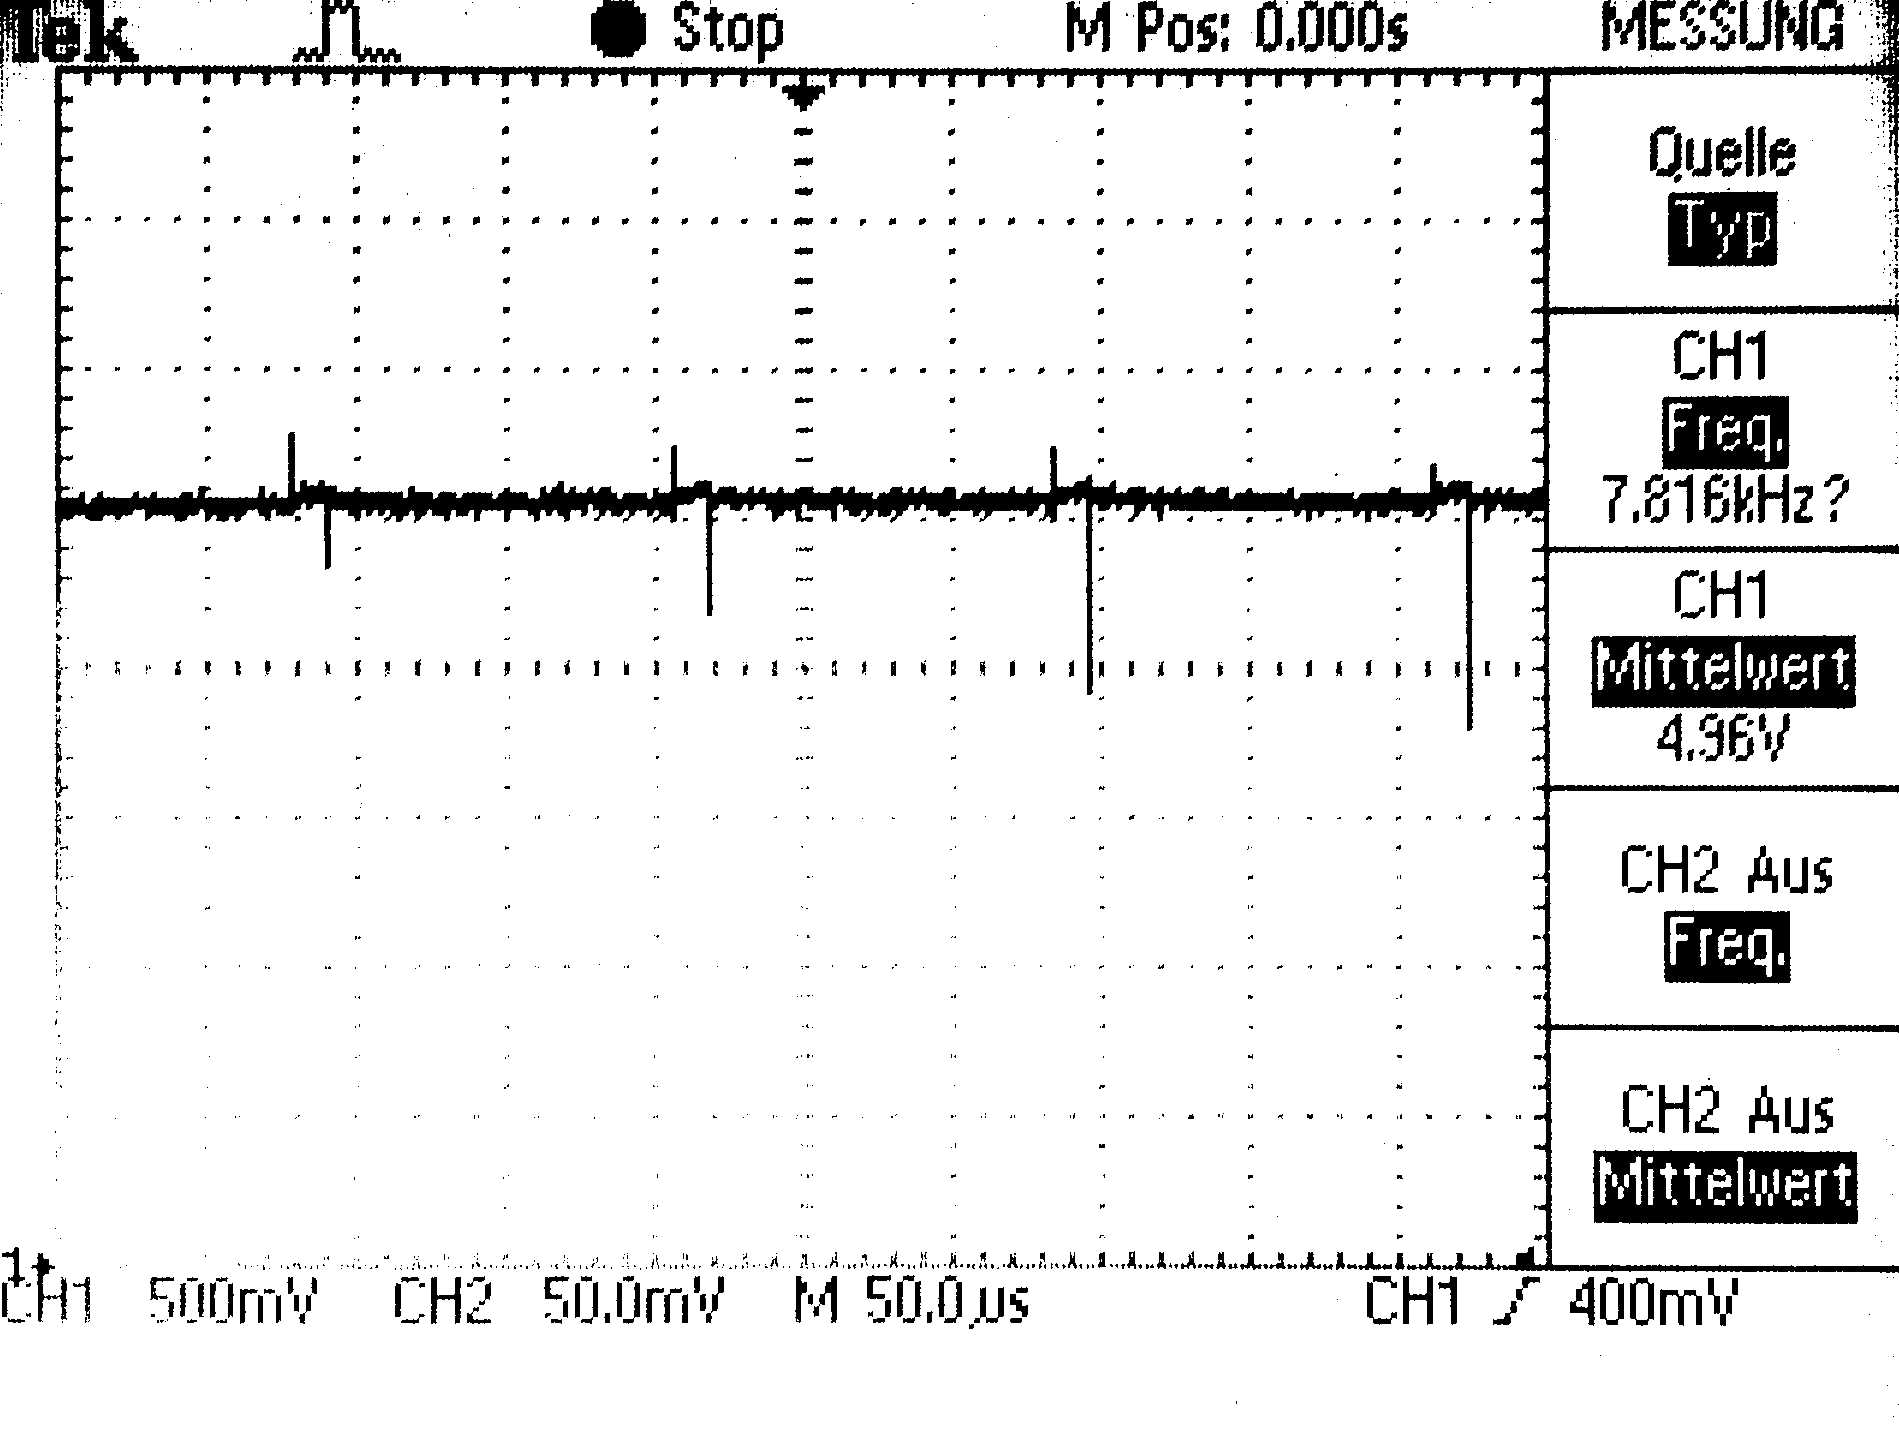
\includegraphics[width=.8\textwidth]{5V_supply.png}\\
\caption{Störungen im 5V Netz}%
\label{fig:5V Supply}
\end{figure}

Betrachtet man den Verlauf der Spannung im 5V-Netz lässt sich leicht erkennen, dass das Signal von einem dem Strom sehr ähnlichen Signal überlagert wird.
Eine solche Störung kann nur von der Betriebsspannung kommen, da der Motor nicht an das 5V-Netz angeschlossen ist. Scheinbar ist der 5V-Schaltregler nicht in der Lage diese Störungen vollständig auszugleichen.
Daher wird nun die Betriebsspannung untersucht um das Ausmaß der Störungen Beurteilen zu können.
Die Werte wurden in einer 1:10 Teilung gemessen, daher sind alle Spannungen mit dem Faktor 10 zu multiplizieren.

Im Akkubetrieb (\cref{fig:accu_supply}) kann gut Beobachtet werden, dass die Spannung um mehr als \SI{100}{\mV} schwankt. Die Frequenz der Spannungseinbrüche entspricht in etwa
der PWM Frequenz von \SI{7812,5}{\hertz}.  Der Motor wurde währenddessen mit einem Tastgrad von 30:256 Angesteuert und wurde nicht belastet.


\begin{figure}[H]
\centering
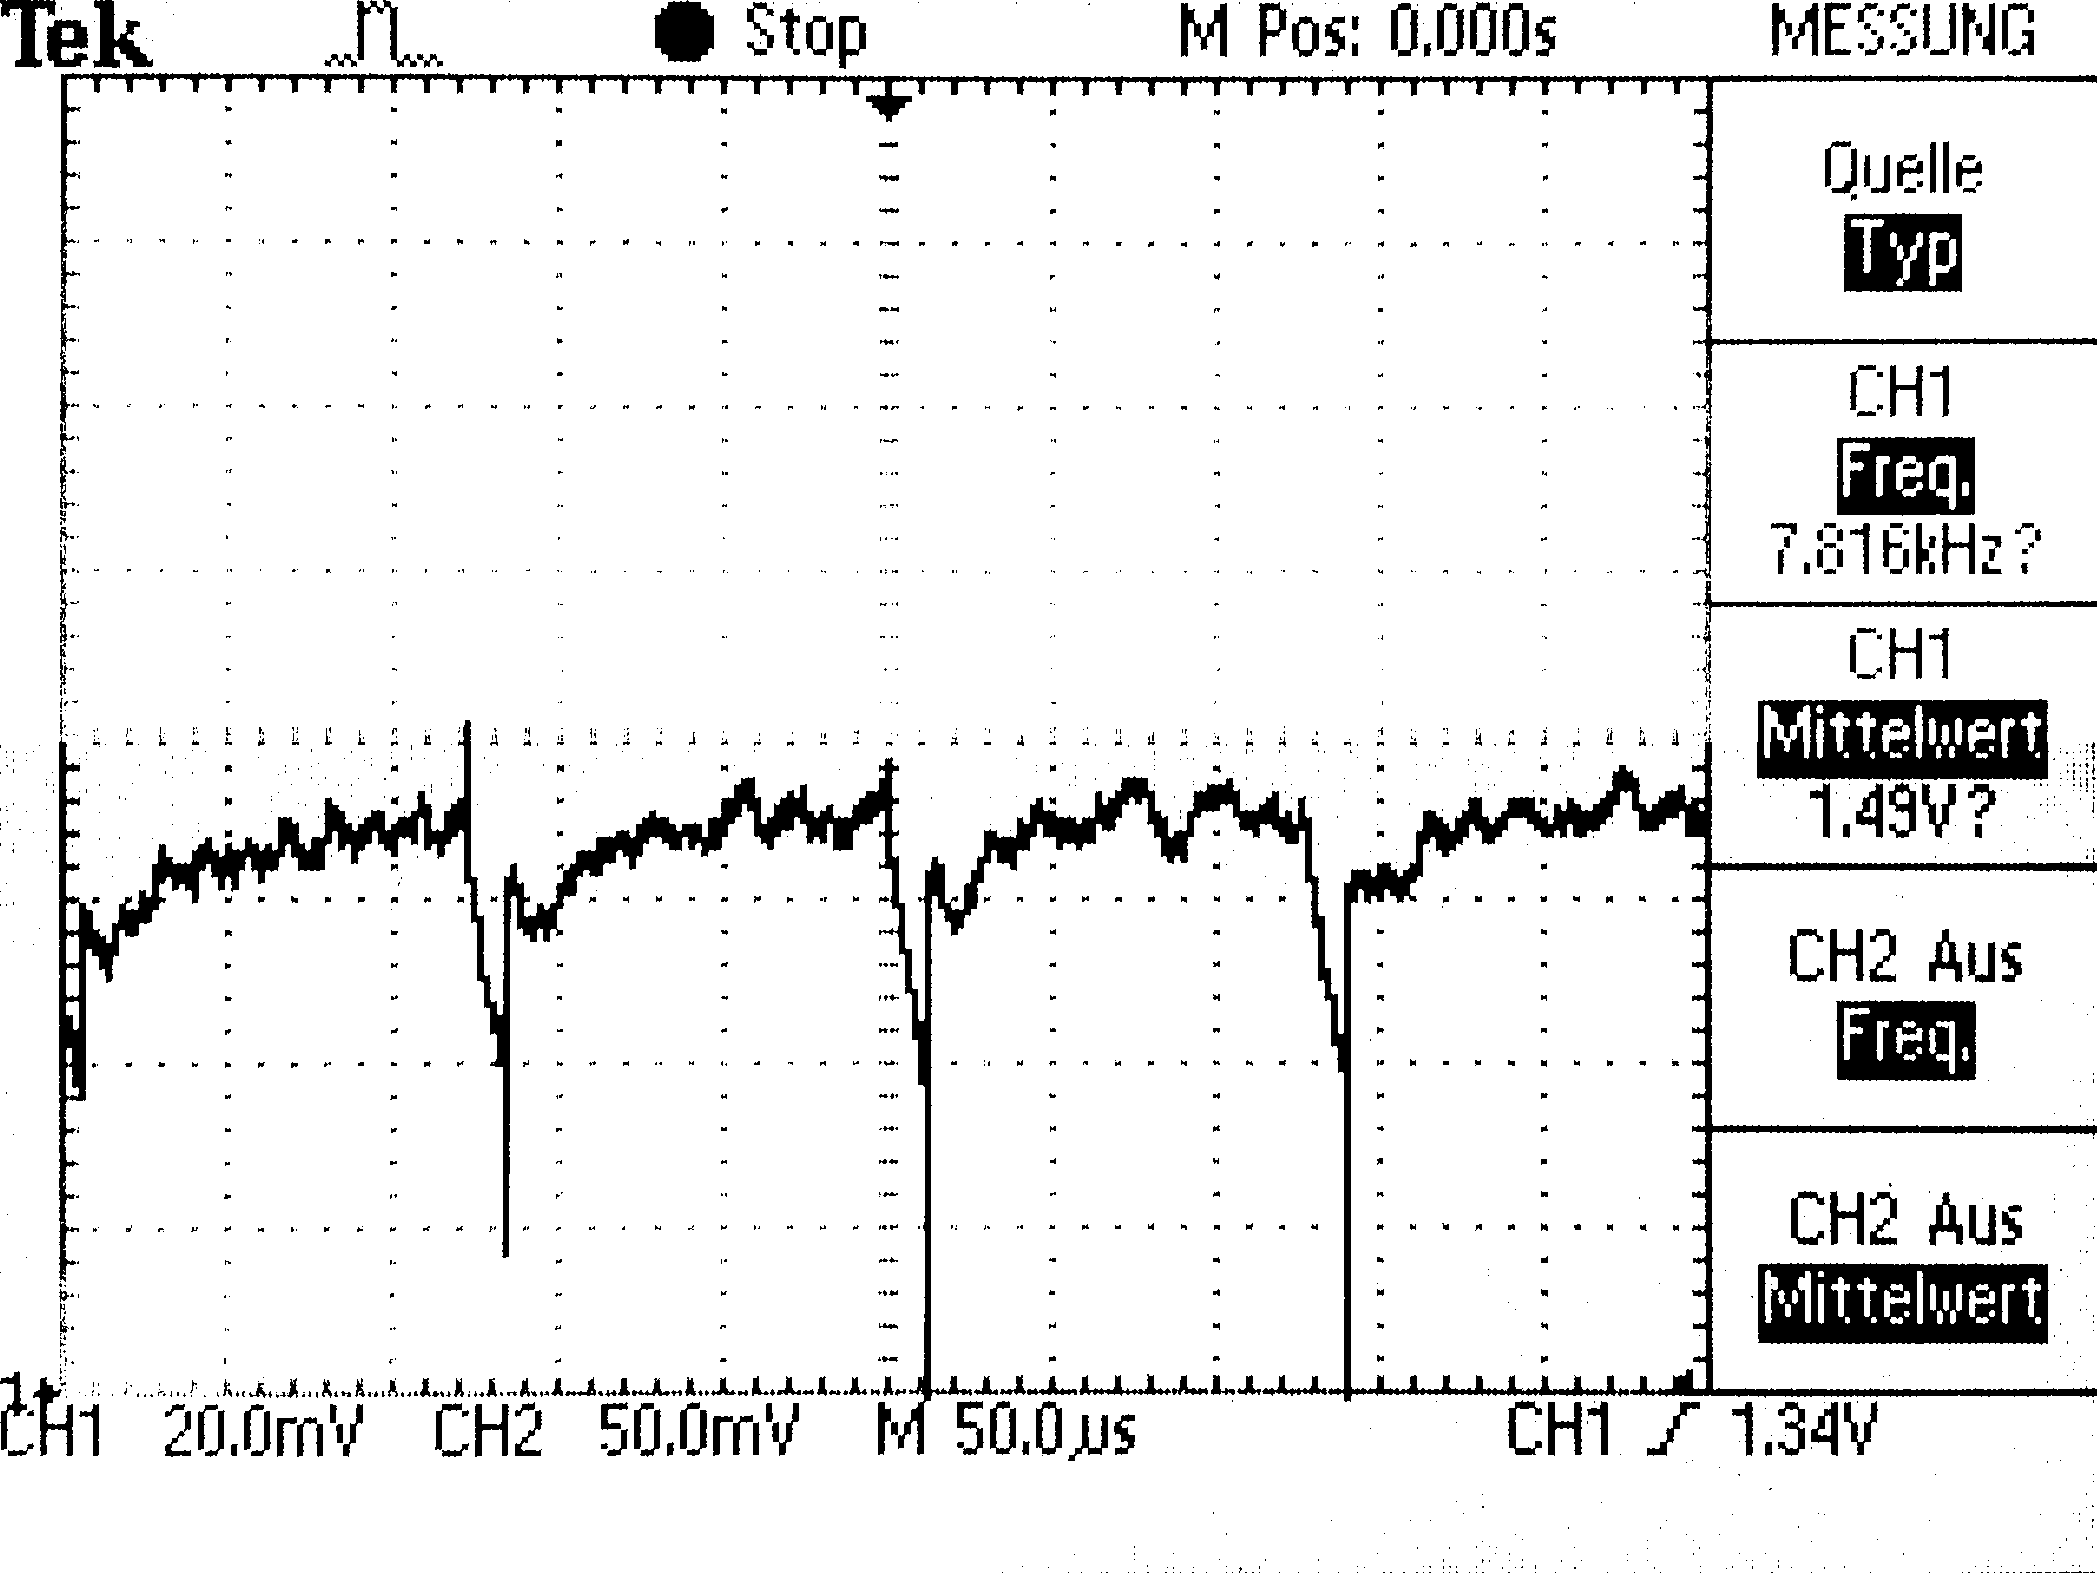
\includegraphics[width=.8\textwidth]{VCC_AKKU.png}\\
\caption{Störungen der Betriebsspannung mit Akku}%
\label{fig:accu_supply}
\end{figure}


Vergleicht man die Messungen im Akkubetrieb mit den Messungen im Netztbetrieb (\cref{fig:power_supply}), kann man erkennen das das Netzteil versucht die Schwankungen auszugleichen.

\begin{figure}[H]
\centering
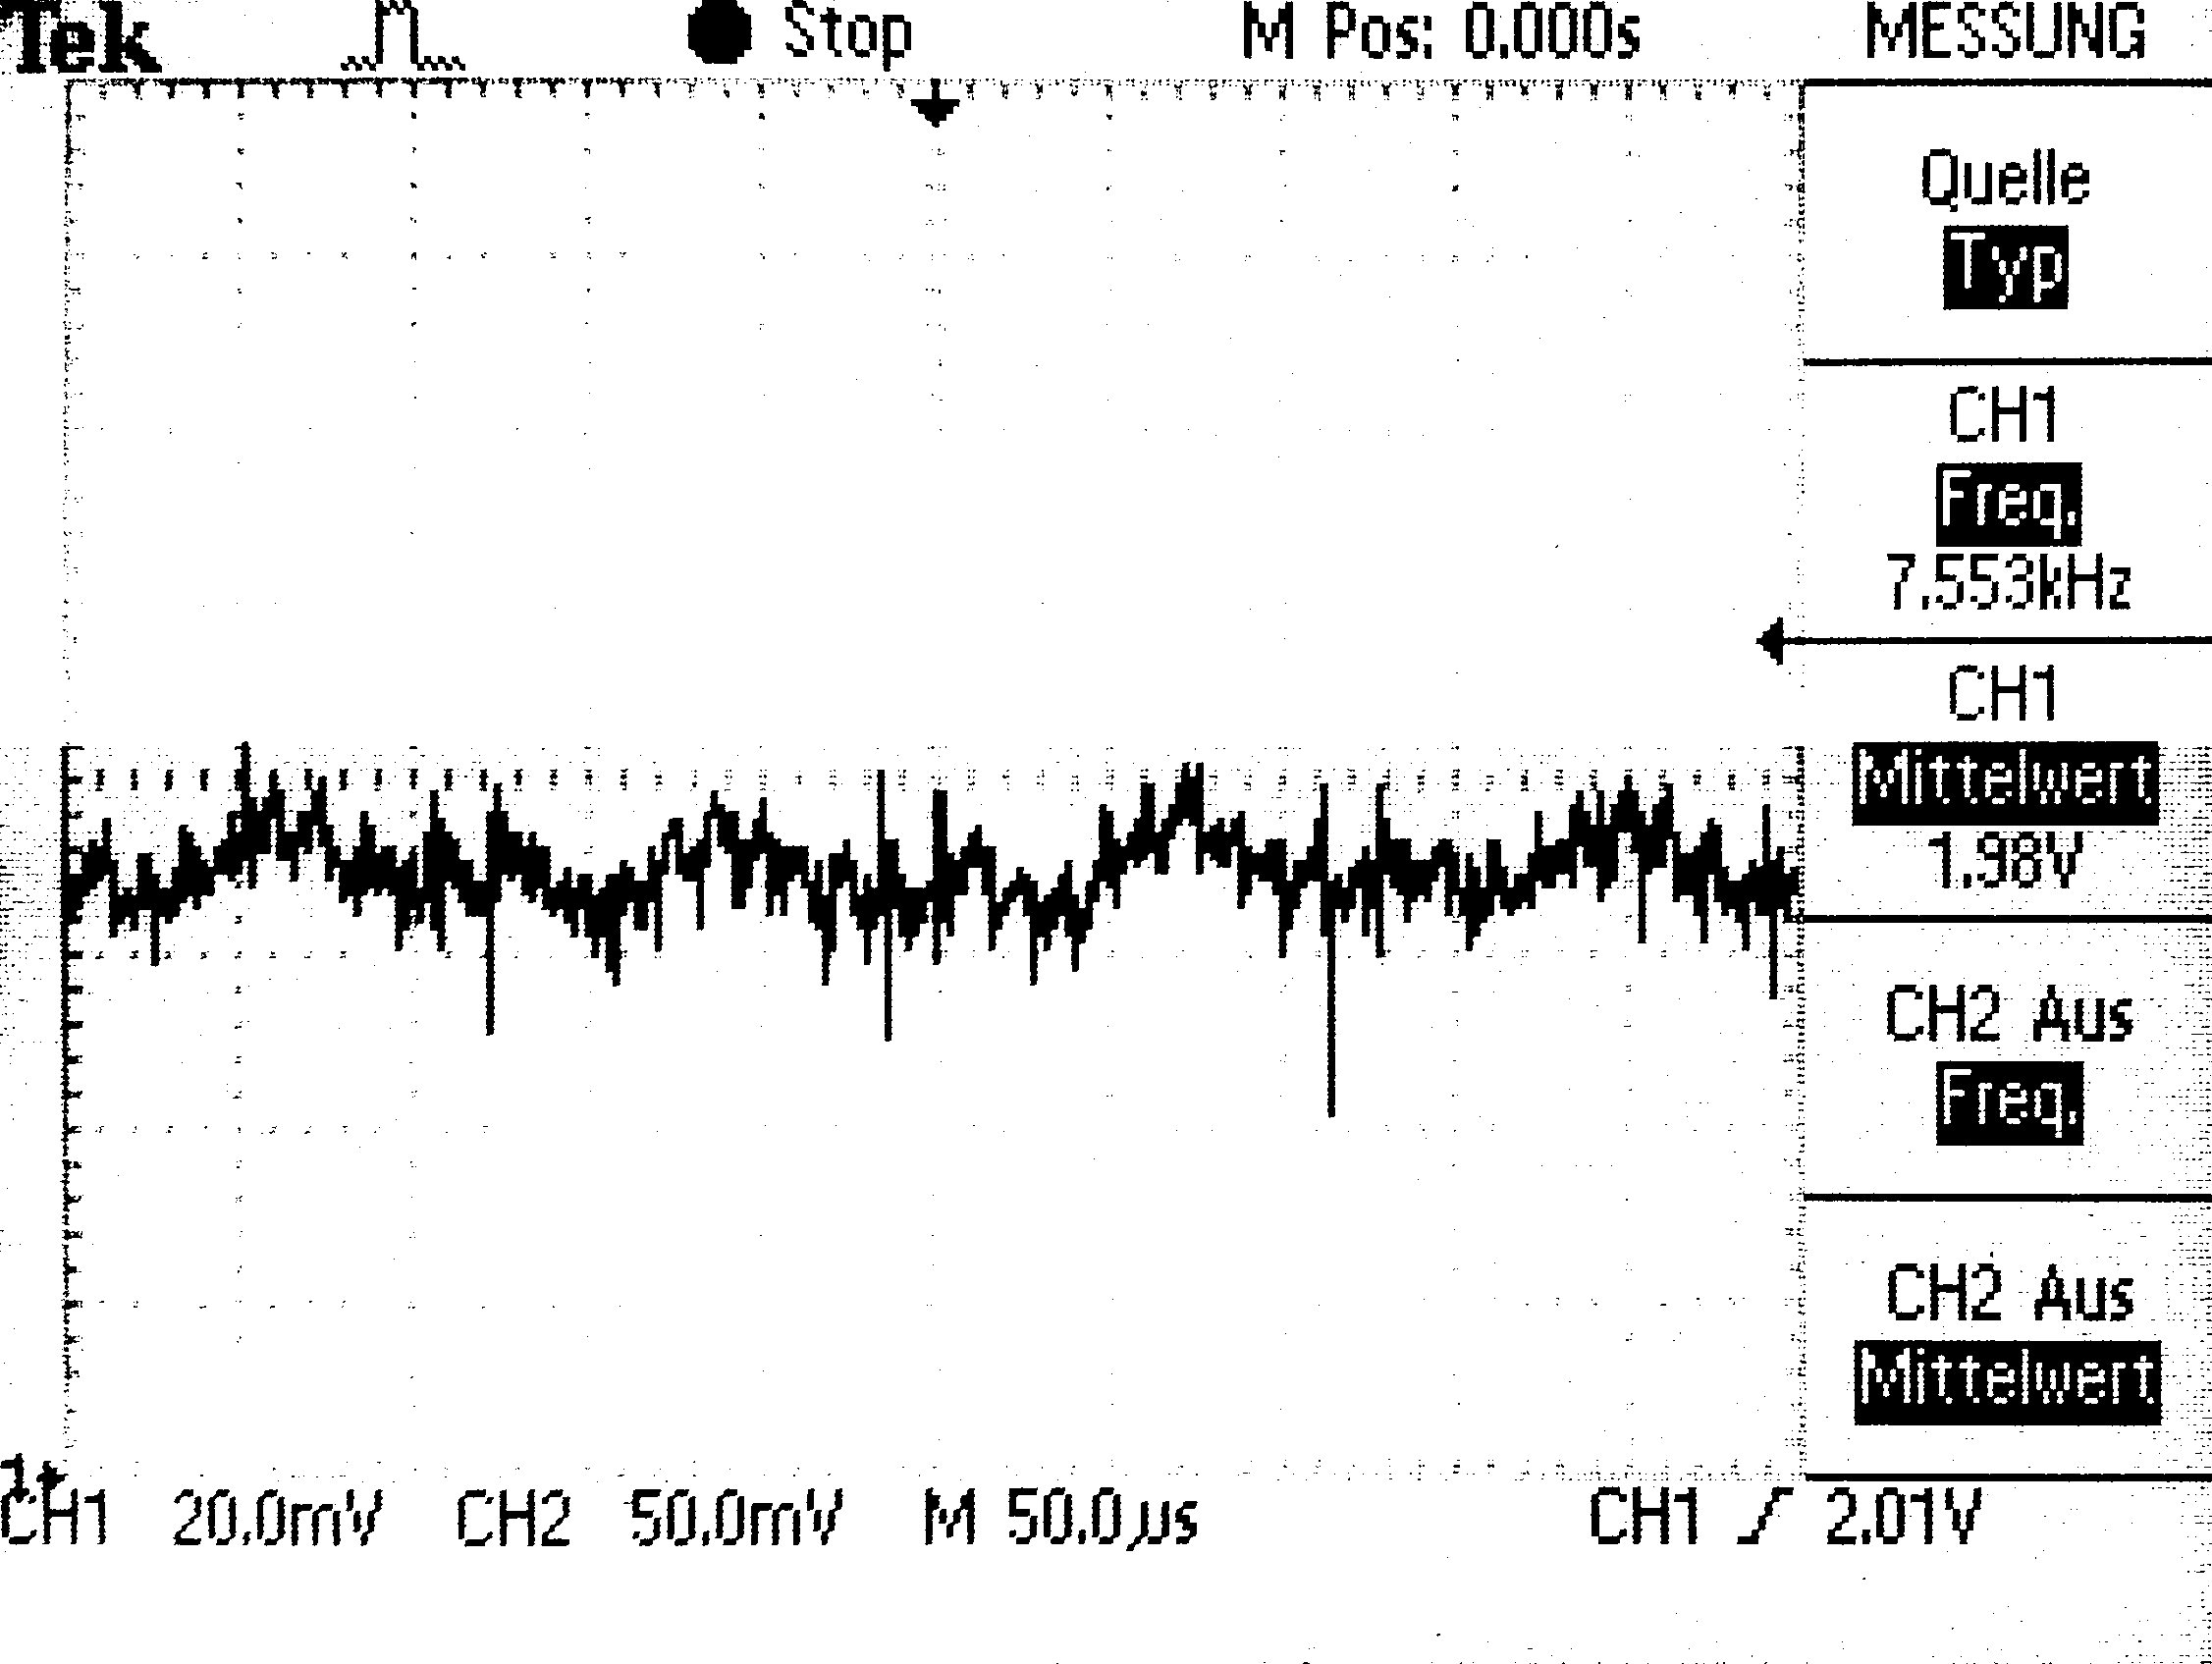
\includegraphics[width=.8\textwidth]{VCC_SUPPLY.png}\\
\caption{Störungen der Betriebsspannung mit Netzteil}%
\label{fig:power_supply}
\end{figure}

Unter Last bei einem Tastgrad von 50:256 betägt die Amplitude der Schwankungen im Akkubetrieb über 3V. Die Messung wurde ohne 1:10 Teilung durchgeführt.
Erstaunlicherweise war trotz der starken Schwankungen noch ein stabiler Betrieb des Fahrzeuges möglich. Dies wurde jedoch nur ca 30sec getestet, denn
die hohe Belastung führte zu einer starken Wärmeentwicklung des Motors.

\begin{figure}[H]
\centering
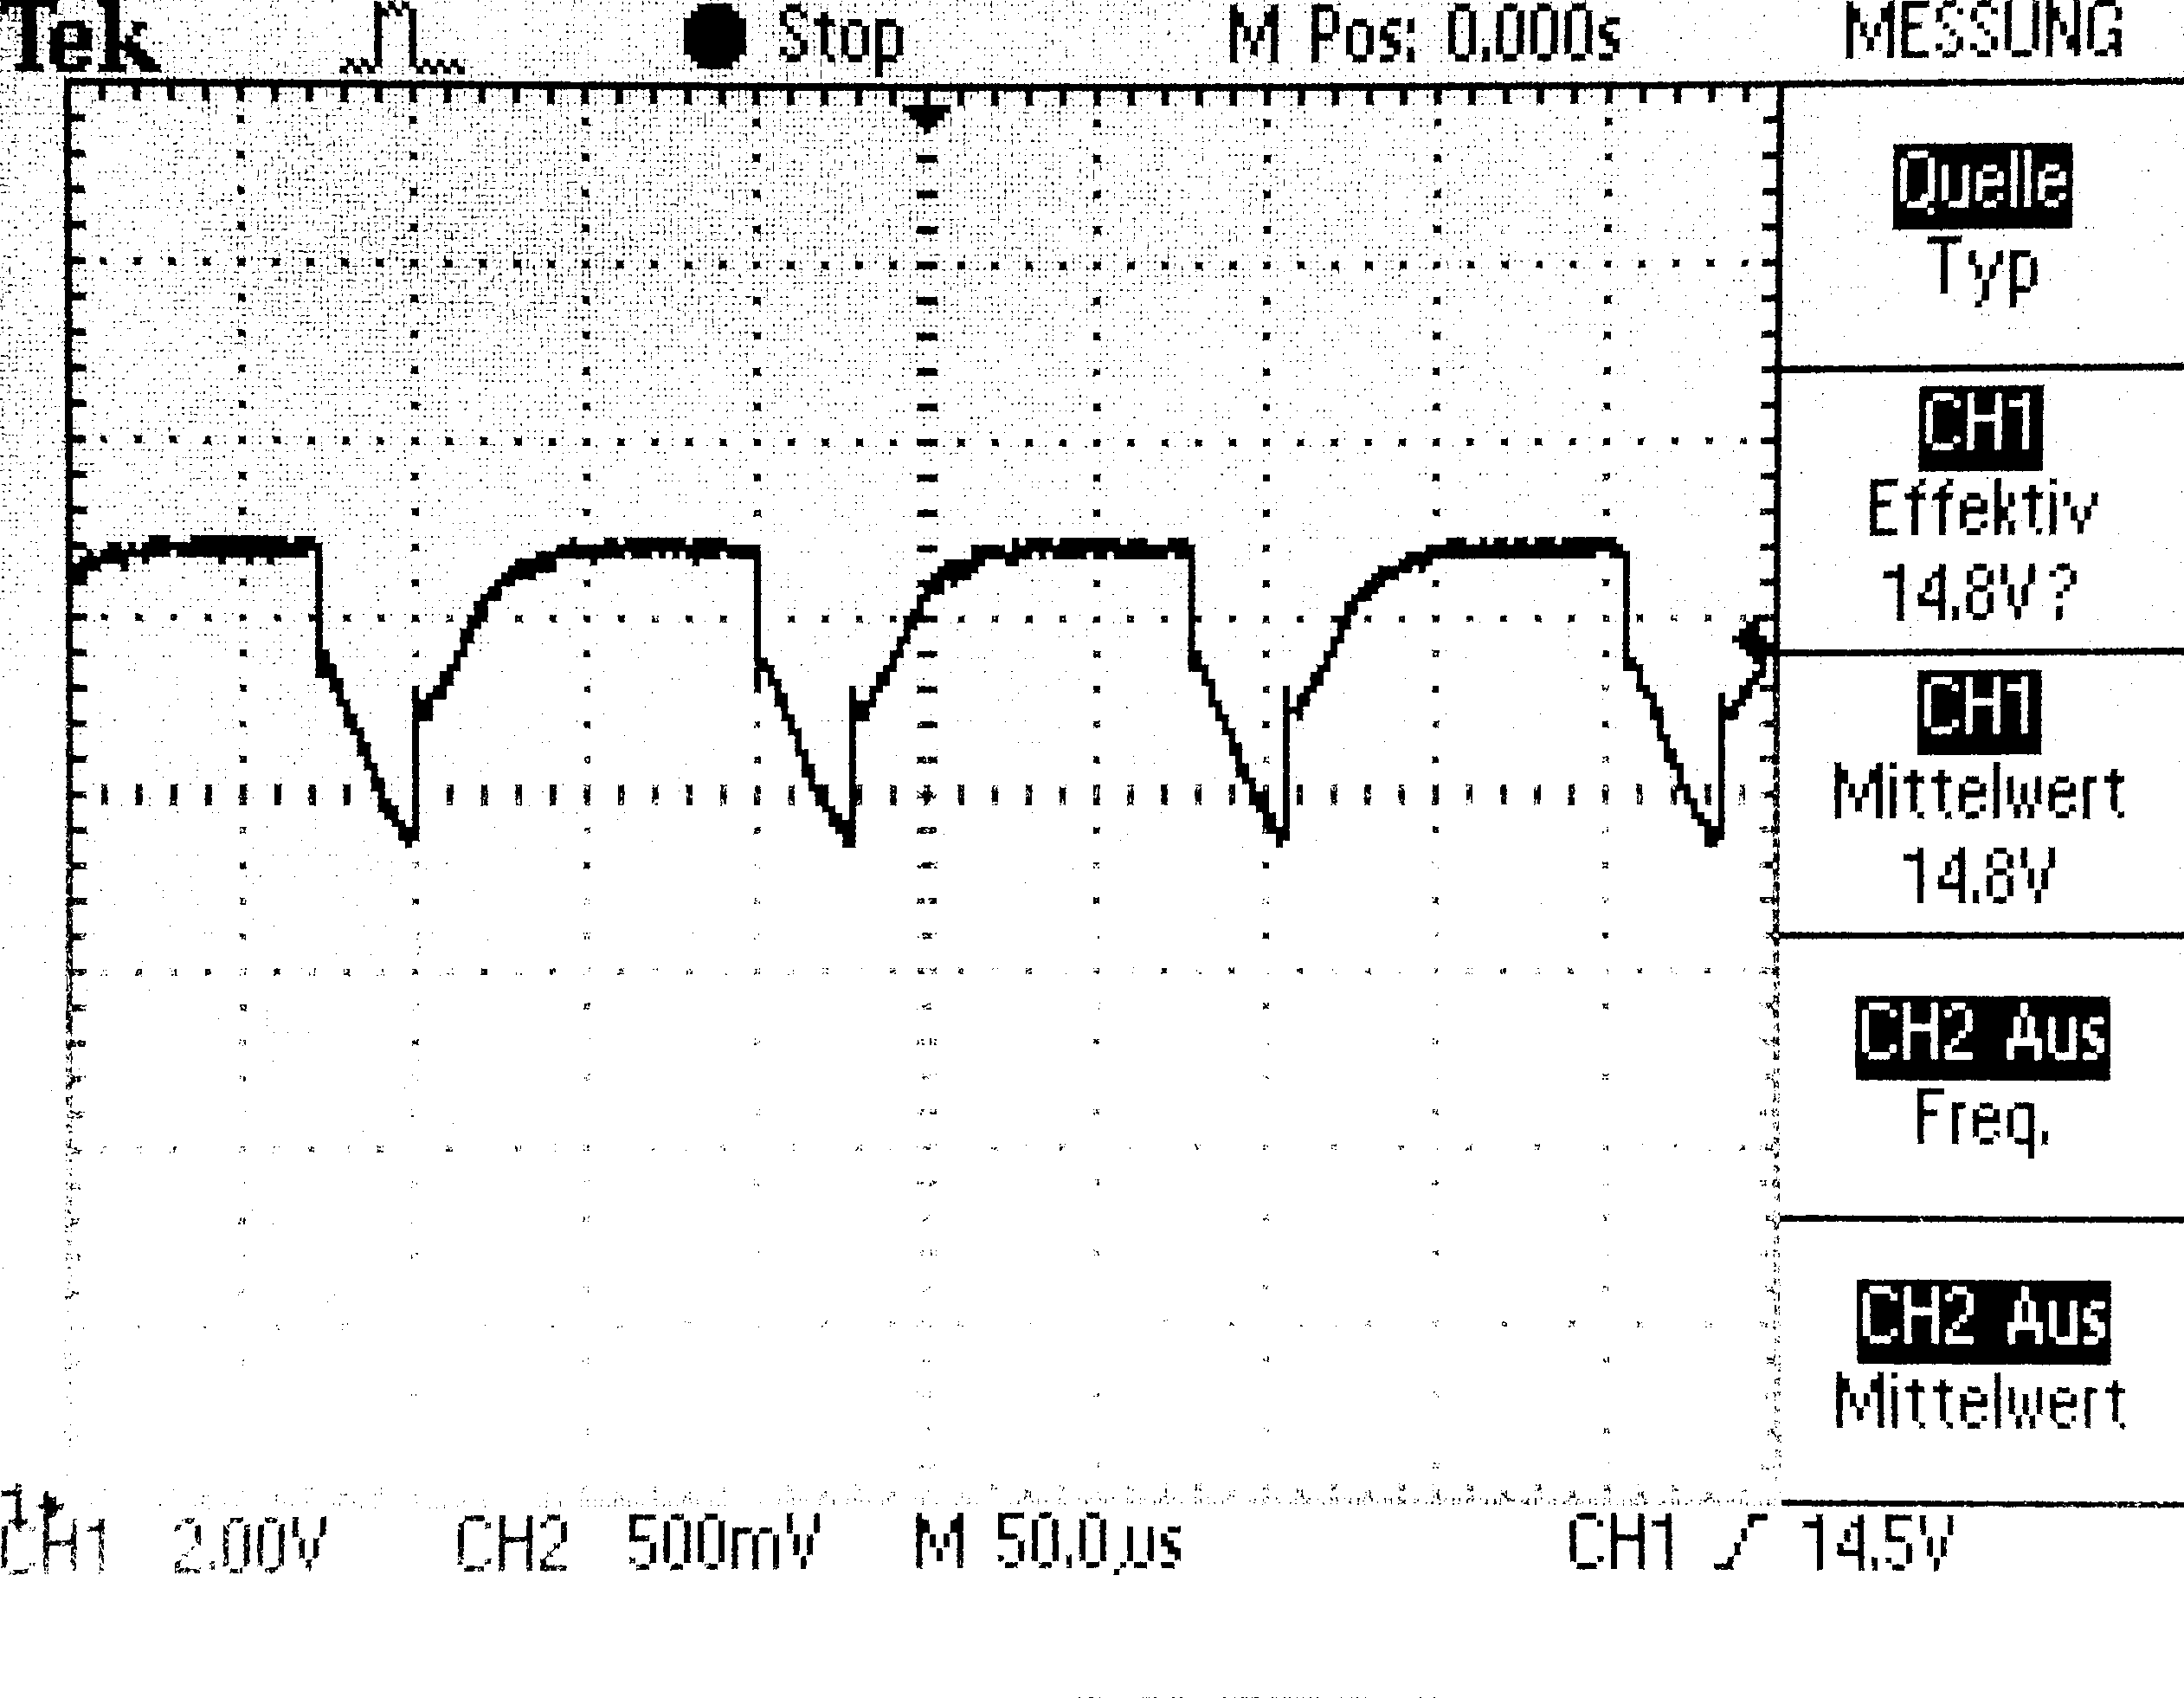
\includegraphics[width=.8\textwidth]{VCC_AKKU_LAST.png}\\
\caption{Störungen der Betriebsspannung mit Akku unter Last}%
\label{fig:power_supply}
\end{figure}

Betrachet man das 5V-Netz unter diesen Bedingungen (\cref{fig:5V_last}) zeigt sich die beeindruckende Leistung des 5V Schaltreglers.
Das 5V-Netz scheint troz der immensen Störung stabiler zu sein als bei niedriger Motorlast. 

\begin{figure}[H]
\centering
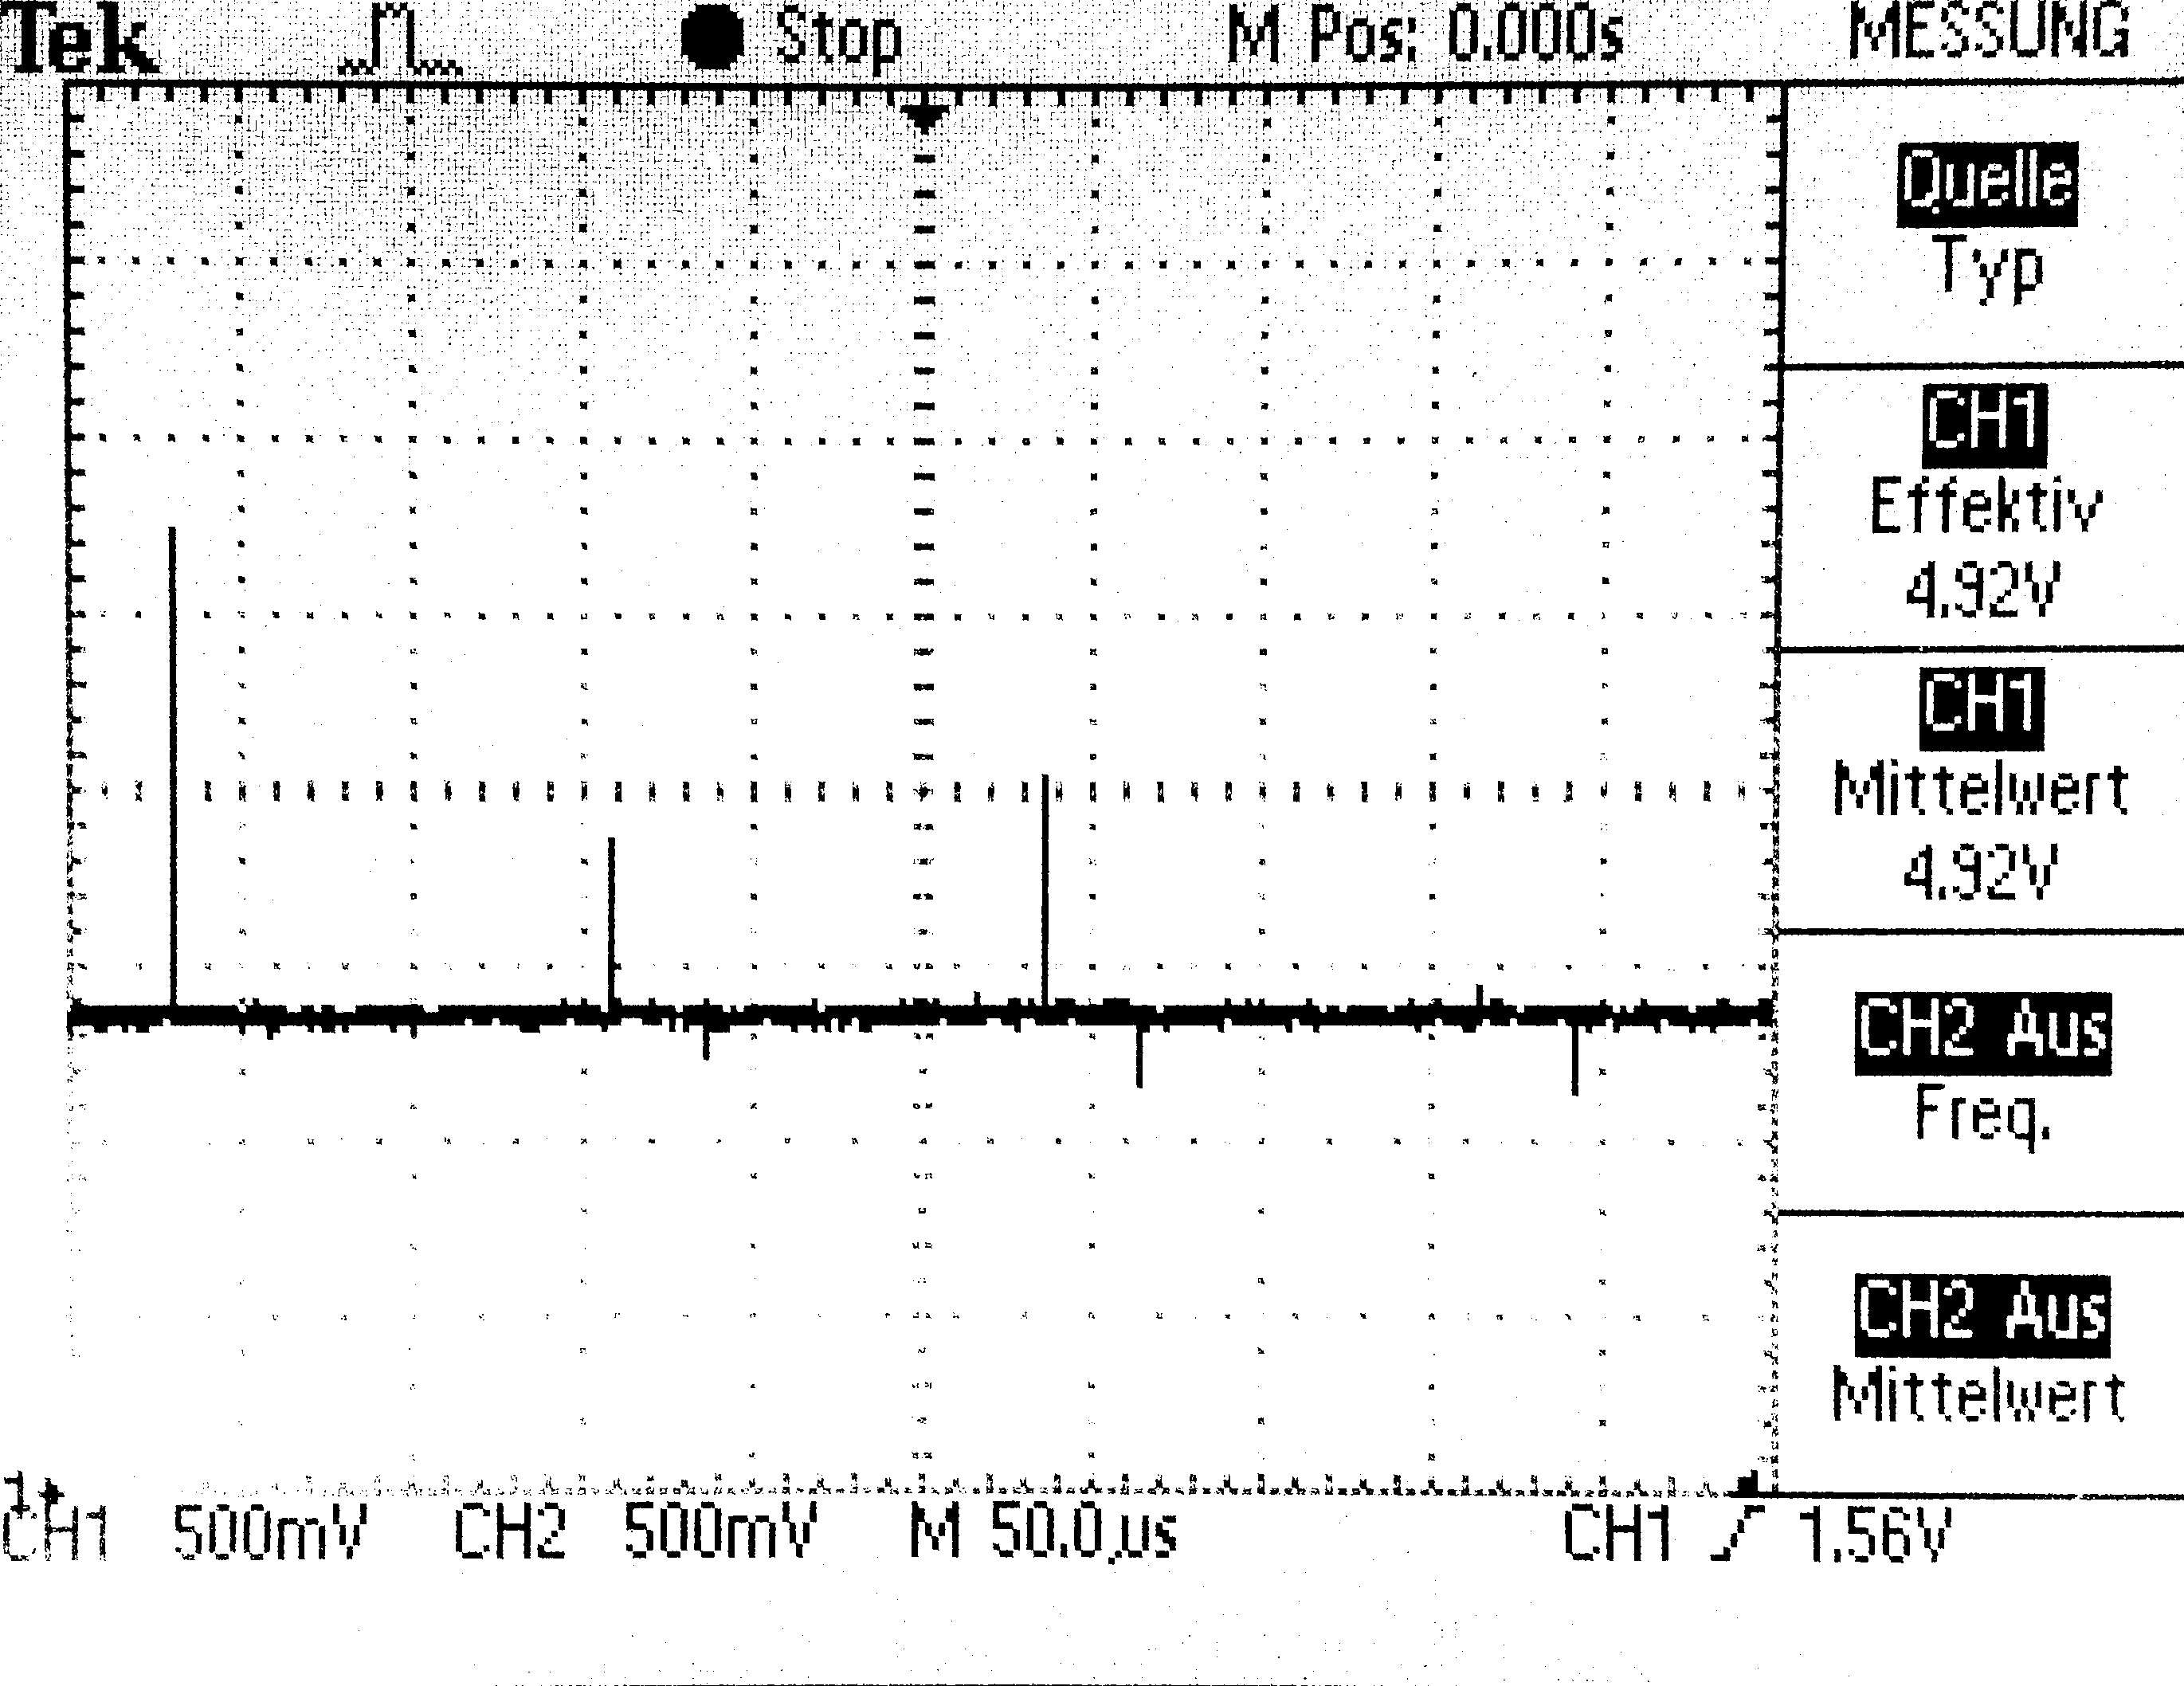
\includegraphics[width=.8\textwidth]{5V_LAST.png}\\
\caption{Störungen des 5V Netzes unter Last}%
\label{fig:5V_last}
\end{figure}

Da das 5V Netz auch unter Last stabil bleibt, sind auch bei höheren Motorlasten keine größeren Störungen in den Sensormesswerten zu erwarten.


\section{Inertisalsensor}

Da die Auswertung der Inertialsensorik ist nicht teil diese Arbeit. Um jedoch die Abhängigkeit der Inertialsensorik von der Motorlast
zu untersuchen, wurden einige Messwerte aufgenommen.

Die Messwerte wurden unter Last bei dem angegebenen Tastgrad aufgenommen. Um die Anzahl der Messwerte gering zu halten wurde legendlich die x-Achse der Sensoren untersucht.

\begin{table}[H]
  \centering
  \begin{tabularx}{\textwidth}{|X|r|r|}
    \hline
     Tastgrad & Erwartungswert [\SI{}{\metre\per\second\squared}] & Standardabweichung [\SI{}{\metre\per\second\squared}]  \\ \hline \hline
     20 & -0.02034  & 0.00078 \\ \hline
     30 & -0.02047  & 0.00225 \\ \hline
     40 & -0.02035  & 0.00097 \\ \hline
     50 & -0.02034  & 0.00074 \\ \hline
     60 & -0.02028  & 0.00189 \\ \hline
  \end{tabularx}
  \caption{Accelerometer}%
  \label{tab:acc}
\end{table}

\begin{table}[H]
  \centering
  \begin{tabularx}{\textwidth}{|X|r|r|}
    \hline
     Tastgrad & Erwartungswert [\SI{}{\radian\per\second}] & Standardabweichung [\SI{}{\radian\per\second}]  \\ \hline \hline
     20 & 0.72961 & 0.27632\\ \hline
     30 & 0.77174 & 0.30825\\ \hline
     40 & 0.78556 & 0.27121\\ \hline
     50 & 0.77792 & 0.27066\\ \hline
     60 & 0.87919 & 0.23369\\ \hline
  \end{tabularx}
  \caption{Gyroskop}%
  \label{tab:gyro}
\end{table}


Sowohl beim Accelerometer als auch beim Gyroskop lässt sich anhand der Daten keine Abhängigkeit erkennen.

\begin{table}[H]
  \centering
  \begin{tabularx}{\textwidth}{|X|r|r|}
    \hline
     Tastgrad & Erwartungswert [\SI{}{\tesla}] & Standardabweichung [\SI{}{\tesla}]  \\ \hline \hline
     20 & 0.06974 & 0.00436\\ \hline
     30 & 0.07602 & 0.00715\\ \hline
     40 & 0.07336 & 0.01154\\ \hline
     50 & 0.06504 & 0.01366\\ \hline
     60 & 0.06564 & 0.01894\\ \hline
  \end{tabularx}
  \caption{Magnetometer}%
  \label{tab:mag}
\end{table}

Beim Magnetometer lässt sich jedoch erkennen, das die Streung der Daten mit zunehmender Motorlast ebenfals zunimmt. Da der Motor jedoch ein Magnetfeld
erzeugt, welches mit zunehmender Belastung zunimmt, war ein Einfluss auf die Messwerte zu erwarten. Diese Störungen sollten bei der verwendung
des Magnetometers beachtet werden.


  %set xrange [0.03:0.04]
  %set yrange [2.62:2.66]
  %set xlabel 'Zeit in [s]'
  %set ylabel 'Spannung in [V]'

\begin{figure}[H]
\centering
\begin{gnuplot}[terminal=pdf]
  set nokey 

  plot 'MessData/Imu-servo/mit_stoerung.csv' with line
\end{gnuplot}
\caption{Restwelligkeit des Filters}
\label{plott:ripple}
\end{figure}

\begin{figure}[H]
\centering
\begin{gnuplot}[terminal=pdf]
  set nokey 

  plot 'MessData/Imu-servo/ohne_stoerung.csv' with line
\end{gnuplot}
\caption{Restwelligkeit des Filters}
\label{plott:ripple}
\end{figure}


\section{Stromverbrauch}

Der Stromverbrauch des Fahrzeugs ist ein wichtiges Kriterium in den statischen Disziplinen. Um den Stromverbrauch im laufenden Betrieb messen zu können, wird hier ein Versuchsaufbau verwendet welcher der Messung des
Motorstomes ähnelt. Die Schaltung besteht dabei aus einem Shuntwiderstand, einer aktiven Filterschaltung und einem Arduino, welcher die Daten zum NUC weiterleitet. Der Vorteil dieser Methode ist, dass die Daten
unter realen Bedingungen in Echtzeit aufgezeichtet werden können. \cref{fig:Strom} zeigt den Verlauf des Stromes währed folgendem Szenario: Bis ca 25s steht das Auto, sämmtliche Software ist dabei auf 
dem Fahrzeug aktiv. Ab 25s beschleunigt das Fahrzeug auf $1,3\frac{m}{s}$ und verhart dort bis ca. Sekunde 57, in welcher es gegen eine Wand fährt. Der grüne Graph stellt dabei den Strom durch den Motor dar, während
der blaue Graph den Gesammtverbrauch des Fahrzeugs darstellt. Die roten Linien Stellen einen gleitenden Mittelwert aus den letzten 200 Messwerten dar. Gut zu erkenn ist, das der Stromverbrauch des Fahrzeugs im Stand unter 
10 Watt liegt. Der Mittelwert des Verbrauches im Stand beträgt 7,9 Watt, während das Fahrzeug in der dar fahrt knapp 13 Watt an Leistung aufnimmt. Nur während das Fahrzeug beschleunigt benötigt es für die Dauer
des Beschleunigungsvorganges mehr Leistung. Fährt das Fahrzeug gegen ein Hinderniss, sodas die Räder blockieren befindet sich der Motor im Kurzschlussbetrieb, dabei reduziert sich sein widerstand auf den Ohmschen widerstand
Motors, was zu einem hohen Stromfluss durch den Motor führt. Dauerhaft kann das durch Überhitzung zur Zerstörung des Motors oder der Treiberplatine führen.


\begin{figure}[H]
\centering
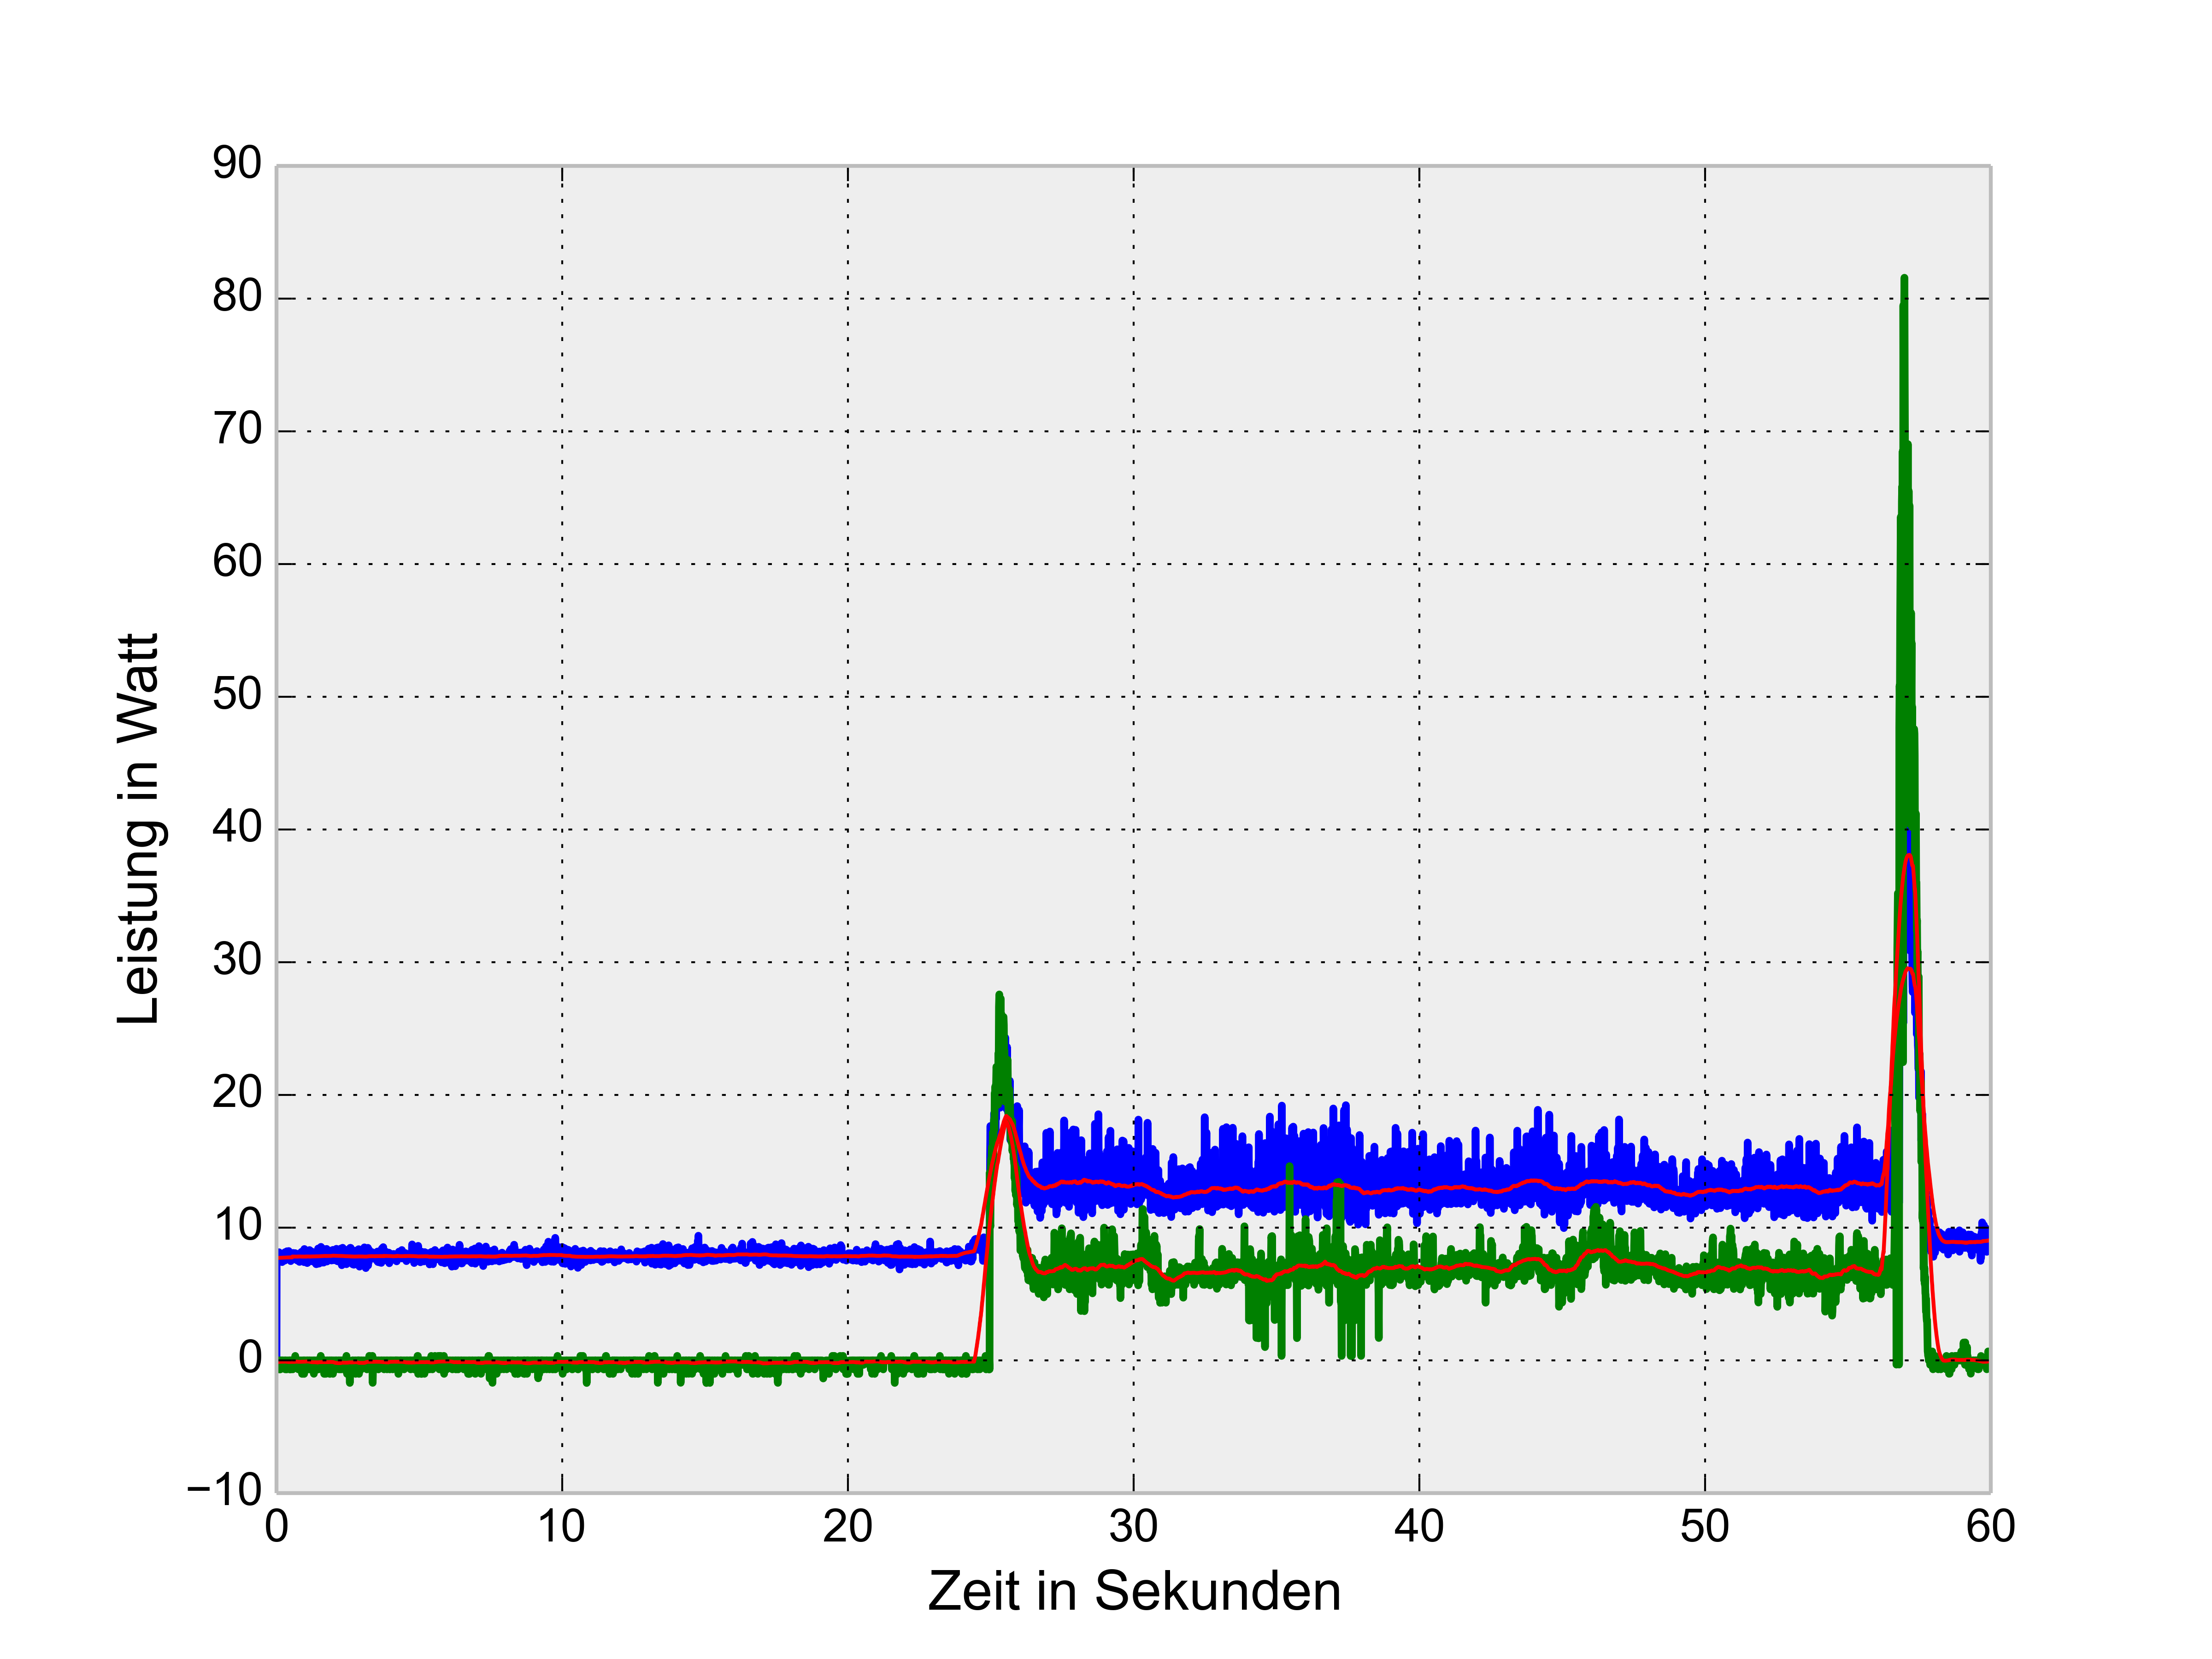
\includegraphics[width=.8\textwidth]{Strom/Power.png}\\
\caption{Salle-Key Tiefpass mit Shunt}%
\label{fig:Strom}
\end{figure}






\section{Infrarotsensoren}

\section{Inertialsensor}

\section{Zeitverhalten der seriellen Verbindung}

Um eine Aussage über das Alter eines Messwertes zu machen. 

\cite{ds-at90can}
adc Wandlung=13Takte
Prescaler=128 bei 16MHz=125000kHz =104uS pro Messung


Bytedauer = 11Bit (1Start+8Daten+2Stopp) 500000Baud --> 22us Bytdauer -> Preamble=5Bytes (4x255+ID) = 110us



\subsection{VoltageCurrent}
25.0319430503
718.591761425


\begin{gnuplot}[terminal=pdf]

  n=70 #number of intervals
  max=872. #max value
  min=596. #min value
  width=(max-min)/n #interval width

  hist(x,width)=width*floor(x/width)+width/2.0

  set xrange [min:max]
  set yrange [0:]

  set offset graph 0.05,0.05,0.05,0.0
  set xtics min,(max-min)/5,max
  set boxwidth width*0.9
  set style fill solid 0.5 #fillstyle
  set tics out nomirror
  set xlabel "x"
  set ylabel "Frequency"
  #count and plot
  plot "MessData/VoltageCurrent.csv" u (hist($1,width)):(1.0) smooth freq w boxes lc rgb"grey" notitle
\end{gnuplot}

\subsection{Distance}
28.1616619788
484.734158193


\begin{gnuplot}[terminal=pdf]

  n=70 #number of intervals
  max=673. #max value
  min=359. #min value
  width=(max-min)/n #interval width

  hist(x,width)=width*floor(x/width)+width/2.0

  set xrange [min:max]
  set yrange [0:]

  set offset graph 0.05,0.05,0.05,0.0
  set xtics min,(max-min)/5,max
  set boxwidth width*0.9
  set style fill solid 0.5 #fillstyle
  set tics out nomirror
  set xlabel "x"
  set ylabel "Frequency"
  #count and plot
  plot "MessData/Distance.csv" u (hist($1,width)):(1.0) smooth freq w boxes lc rgb"green" notitle
\end{gnuplot}


\subsection{Infrared}
35.0709303606
696.91743058



\begin{gnuplot}[terminal=pdf]

  n=70 #number of intervals
  max=825. #max value
  min=586. #min value
  width=(max-min)/n #interval width

  hist(x,width)=width*floor(x/width)+width/2.0

  set xrange [min:max]
  set yrange [0:]

  set offset graph 0.05,0.05,0.05,0.0
  set xtics min,(max-min)/5,max
  set boxwidth width*0.9
  set style fill solid 0.5 #fillstyle
  set tics out nomirror
  set xlabel "x"
  set ylabel "Frequency"
  #count and plot
  plot "MessData/Infrared.csv" u (hist($1,width)):(1.0) smooth freq w boxes lc rgb"green" notitle
\end{gnuplot}


\subsection{uCTime}
31.2060346589
477.761007865



\begin{gnuplot}[terminal=pdf]

  n=70 #number of intervals
  max=685. #max value
  min=366. #min value
  width=(max-min)/n #interval width

  hist(x,width)=width*floor(x/width)+width/2.0

  set xrange [min:max]
  set yrange [0:]

  set offset graph 0.05,0.05,0.05,0.0
  set xtics min,(max-min)/5,max
  set boxwidth width*0.9
  set style fill solid 0.5 #fillstyle
  set tics out nomirror
  set xlabel "x"
  set ylabel "Frequency"
  #count and plot
  plot "MessData/ucTime.csv" u (hist($1,width)):(1.0) smooth freq w boxes lc rgb"green" notitle
\end{gnuplot}

\subsection{Motor}
38.0093527069
391.111706657


\begin{gnuplot}[terminal=pdf]

  n=70 #number of intervals
  max=534. #max value
  min=287. #min value
  width=(max-min)/n #interval width

  hist(x,width)=width*floor(x/width)+width/2.0

  set xrange [min:max]
  set yrange [0:]

  set offset graph 0.05,0.05,0.05,0.0
  set xtics min,(max-min)/5,max
  set boxwidth width*0.9
  set style fill solid 0.5 #fillstyle
  set tics out nomirror
  set xlabel "x"
  set ylabel "Frequency"
  #count and plot
  plot "MessData/motor.csv" u (hist($1,width)):(1.0) smooth freq w boxes lc rgb"green" notitle
\end{gnuplot}




\subsection{IMU}
40.8272894054
3425.96398337


\begin{gnuplot}[terminal=pdf]

  n=70 #number of intervals
  max=3605. #max value
  min=3312. #min value
  width=(max-min)/n #interval width

  hist(x,width)=width*floor(x/width)+width/2.0

  set xrange [min:max]
  set yrange [0:]

  set offset graph 0.05,0.05,0.05,0.0
  set xtics min,(max-min)/5,max
  set boxwidth width*0.9
  set style fill solid 0.5 #fillstyle
  set tics out nomirror
  set xlabel "x"
  set ylabel "Frequency"
  #count and plot
  plot "MessData/imu.csv" u (hist($1,width)):(1.0) smooth freq w boxes lc rgb"green" notitle
\end{gnuplot}


\subsection{Gesammt}
142.365993405
6195.08004809


\begin{gnuplot}[terminal=pdf]

  n=70 #number of intervals
  max=6522. #max value
  min=5574. #min value
  width=(max-min)/n #interval width

  hist(x,width)=width*floor(x/width)+width/2.0

  set xrange [min:max]
  set yrange [0:]

  set offset graph 0.05,0.05,0.05,0.0
  set xtics min,(max-min)/5,max
  set boxwidth width*0.9
  set style fill solid 0.5 #fillstyle
  set tics out nomirror
  set xlabel "x"
  set ylabel "Frequency"
  #count and plot
  plot "MessData/gesammt.csv" u (hist($1,width)):(1.0) smooth freq w boxes lc rgb"green" notitle
\end{gnuplot}